\documentclass[11pt,a4paper]{article}
\usepackage[margin=2.2cm]{geometry}
\usepackage{graphicx,booktabs,float,xcolor,hyperref,xurl}
\usepackage[normalem]{ulem}
\newcommand{\dead}[1]{\textcolor{gray}{\sout{#1}}}
\title{AWI-ESM3 on albedo: why the coupled runs are slow}
\author{Jan Streffing}
\date{Last updated: 2026-09-29}

\begin{document}
\maketitle

\begin{abstract}
The AWI-ESM3 CMIP7 spin-up (TCO95L91 OpenIFS, CORE3 FESOM2 with cavities, LPJ-GUESS, XIOS, 47 nodes) moved from levante to albedo on 2026-09-26 and ran there at 49 to 57\,SYPD, against 83\,SYPD on levante. This report follows why, and how the layout was changed until the model ran faster on fewer nodes. Where we are (2026-09-29): 25 nodes step 2.40\,s per model day (about 99\,SYPD in steady state, 6.1 node-hours per model year against 19.8 in the first albedo legs), with FESOM at 1800\,s and without OpenMP threads, its 768 ranks spread 96 per node, XIOS and the runoff mapper on the OpenIFS nodes, and OpenIFS and FESOM now sharing the critical path. The steps are in Section~\ref{sec:timeline}, the current state and open questions in Section~\ref{sec:state}, falsified explanations in Section~\ref{sec:falsified}.
\end{abstract}

\section{The campaign, in the order it happened}\label{sec:timeline}

\subsection{First albedo legs (2026-09-26--27)}
After the OASIS partition fix and the OpenIFS cold-start fix, the first clean 10-year legs on albedo took 4\,h\,20\,min to 4\,h\,40\,min of wall time (jobs 47456102, 47472034, 47472035). Levante had done the same legs in about 3\,h. Four other legs died in an XIOS server with a SIGBUS; that problem is documented separately (\texttt{xios\_sigbus\_albedo\_report\_2026-09-28.md}) and is not part of the speed question.

\subsection{Albedo against levante, same configuration (2026-09-28)}
We compared the finished ccnice leg 2110--2119 on albedo (job 47472034) with levante's leg 2090--2099 (job 27681023). Both used 47 nodes with FESOM $1792\times1$, OpenIFS $384\times4$, LPJ-GUESS $64\times8$, XIOS $16\times128$, identical namelists (\texttt{whichEVP}=1, $\alpha=\beta=300$, \texttt{linfs}, cavities) and single-precision OpenIFS on both machines.

\begin{table}[H]\centering\small
\begin{tabular}{lrrr}\toprule
 & levante & albedo & ratio\\\midrule
Leg wall time (s) & 10385 & 15483 & 1.49\\
OpenIFS wall per step (s) & 0.118 & 0.173 & 1.47\\
OpenIFS CPU per step, 4 threads (s) & 0.452 & 0.548 & 1.21\\
FESOM ocean (s per leg) & 4406 & 5694 & 1.29\\
\quad vertical mixing & 1111 & 1304 & 1.17\\
\quad tracer advection & 933 & 1128 & 1.21\\
\quad ssh solver & 1314 & 1850 & 1.41\\
FESOM ice EVP & 2725 & 4992 & 1.83\\
FESOM waiting for the atmosphere (\texttt{ice read forc}) & 441 & 1200 & \\
FESOM output (means and XIOS send) & 1925 & 1831 & 0.95\\\bottomrule
\end{tabular}
\caption{Timings per 10-year leg. FESOM numbers are rank-0 means from its \texttt{MODEL RUNTIME per task} block; OpenIFS from \texttt{ifs.stat} time stamps.}
\end{table}

\begin{figure}[H]\centering
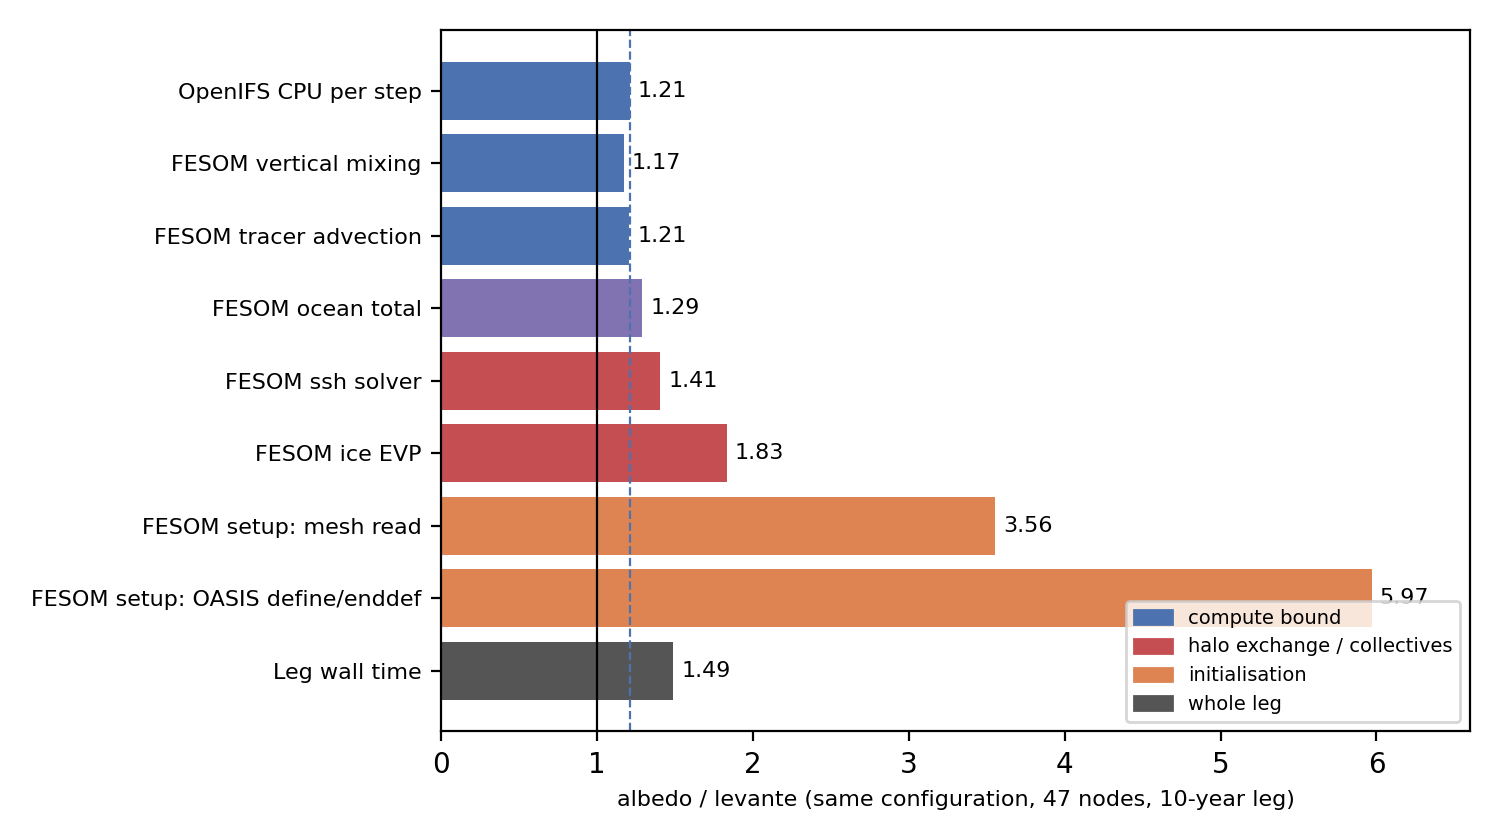
\includegraphics[width=0.9\textwidth]{fig_albedo_vs_levante.png}
\caption{Albedo over levante for the same configuration. Compute-bound parts (blue) slow down by about 20\,\%, the dashed line; a cache-resident benchmark kernel measures levante's Zen3 cores (EPYC 7763, 2449\,MHz under full load) as 16\,\% faster than albedo's Zen2 cores (EPYC 7702, 2331\,MHz). Parts dominated by halo exchanges and collectives (red) slow down by 41 to 83\,\%, and the communication-heavy OASIS setup (orange) by a factor of six. The whole leg is 1.49 times slower.}
\end{figure}

The build is not the cause: both machines use the Intel compiler (ifort 2021.6 on albedo, 2021.5 on levante) with the same base flags, and albedo adds \texttt{-march=core-avx2 -qopt-malloc-options=2 -qopt-prefetch=5 -unroll-aggressive}, which levante does not have. Both machines have HDR100 InfiniBand.

\subsection{Load balance on albedo from logs (2026-09-28)}
This first estimate is superseded by LUCIA below. OpenIFS spends 0.143\,s of CPU per step on its 4 threads (0.571 over 4) out of a 0.173\,s step, so it computes 83\,\% of the time. FESOM is busy 98.5\,\% of the wall time when its \texttt{diag} (2.8\,\%) and \texttt{output} (12.1\,\%) categories are counted, of which 7.9\,\% is the wait for the atmosphere. Both models are saturated and FESOM is the marginally slower one. The daily LPJ-GUESS exchange costs 1.7\,\% (the step after it takes 0.242\,s against 0.17\,s), and there are no year-end stalls: every model year takes 1471 to 1645\,s.

\subsection{Comparison with Miguel's 100-SYPD runs (2026-09-28)}
The albedo sheet of \texttt{AWIESM3-Performance.ods} lists 100.26\,SYPD for FESOM $1792\times2$, OpenIFS $384\times4$ on CORE3Cav, measured over steps 3--1416. Over the same window our leg runs at 53.2\,SYPD. Two differences account for the gap:
\begin{itemize}
\item CMIP7 output. OpenIFS FullPos (\texttt{DYNFPOS} 16.9\,\%, \texttt{GRIDFPOS} 4.7\,\%, \texttt{SU4FPOS} 2.9\,\%) is 24.5\,\% of OpenIFS CPU for 209 files and 42\,GB per model year. Without it the step would be about 0.108\,s. This output is required.
\item FESOM at one thread. Miguel ran FESOM with two OpenMP threads, twice our FESOM cores, which removes the wait of OpenIFS on the ocean.
\end{itemize}
Miguel's run directories are not readable for us (mode 700), so FESOM's own timing in his runs is unknown.

\subsection{XIOS is not a bottleneck (2026-09-28)}
From the XIOS performance reports of the finished leg: the eight first-level servers are busy 2.6 to 2.8\,\% of the time, the eight second-level (file-writing) servers 34 to 41\,\%. The client ratio is 0.74\,\% on OpenIFS rank 0 and 0.04\,\% on FESOM rank 0. XIOS occupies 16 of 47 nodes with one server each, which is the one clear waste of node hours.

\subsection{Initialisation is five times slower (2026-09-28)}
A 1-day test leg (TEST\_xios1d) takes 9\,min: 5.5\,min initialisation, 57\,s of integration and 2.5\,min for finalisation, tidy and the next leg's preparation. File movement is threaded (127 threads) and takes about 20\,s. FESOM's setup timer is the dominant part:

\begin{table}[H]\centering\small
\begin{tabular}{lrrr}\toprule
FESOM setup on rank 0 (s) & levante (3 legs) & albedo (4 legs) & ratio\\\midrule
mesh and partition read & 18--21 & 66--70 & 3.5\\
restart read & 7--8 & 20--40 & 2.5\\
other: OASIS define and \texttt{oasis\_enddef} & 37--38 & 223--234 & 6\\
total & 64--68 & 313--335 & 5\\\bottomrule
\end{tabular}
\caption{The file reads slow down like GPFS I/O; the OASIS router setup, an all-to-all between 1792 and 384 ranks, slows down like the other communication-heavy parts. \texttt{oasis\_enddef} also waits for the slowest model to finish its own initialisation, so part of it may be LPJ-GUESS or OpenIFS input on GPFS.}
\end{table}

\subsection{Node-to-node spread (2026-09-28)}
The ccnice leg 2120--2129 (job 47473364) ran at 0.202\,s per OpenIFS step (48.9\,SYPD) against 0.173\,s in the leg before, with the same configuration on a different set of nodes.


\subsection{TEST\_perfA: FESOM with two threads (2026-09-28)}
A 2-month leg with FESOM $1792\times2$ (61 nodes) ran at 0.149\,s per OpenIFS step (66.4\,SYPD) against 0.176\,s (56.0\,SYPD) with one thread. FESOM's compute per OpenIFS step fell only 8\,\% (0.145 to 0.134\,s): the EVP by 23\,\%, the ocean by 7\,\%, while the ssh solver got 20\,\% slower. Doubling FESOM's cores therefore buys little; FESOM at 1792 ranks is limited by communication, not by arithmetic. (Hardware counters later showed that memory bandwidth is not the limit either, Table~\ref{tab:pmc}.) FESOM's setup took 133\,s in this run against 313 to 335\,s in all earlier albedo runs (mesh read 22 against 66--72\,s), with the same files on the same filesystem, so the initialisation cost varies from job to job.

\subsection{LUCIA: FESOM is the limiter (2026-09-28)}
With \texttt{oasis3mct.use\_lucia: true} OASIS3-MCT 5 writes \texttt{load\_balancing\_info.txt} and one \texttt{timeline\_<component>.nc} per component into the work directory. For TEST\_perfA:
\begin{table}[H]\centering\small
\begin{tabular}{lrr}\toprule
component & computing (s) & waiting (s)\\\midrule
FESOM & 190.7 & 19.2\\
OpenIFS & 92.8 & 125.4\\
LPJ-GUESS & $\approx 0$ & 300.9\\\bottomrule
\end{tabular}
\caption{2-month leg, 1416 OpenIFS steps. The OpenIFS numbers of this summary turned out to be wrong; see the timeline analysis later in this section, which gives 186\,s computing and 54\,s waiting. The CPU column of \texttt{ifs.stat} counts MPI busy-waiting as CPU time, which is why the log-based estimate above put OpenIFS at 83\,\%. The SYPD line of the LUCIA summary is broken (\texttt{*****}); the compute and wait columns add up to the wall time and are sound.}
\end{table}

\subsection{What changed since August (2026-09-28)}
The August albedo runs under \texttt{/albedo/work/user/jstreffi/runtime/awiesm3-develop/} (awiesm3sp\_lucia and relatives, 1 month each, FESOM $1792\times1$ on the same CORE3 mesh with cavities) used a different FESOM configuration:
\begin{table}[H]\centering\small
\begin{tabular}{lll}\toprule
 & August (awiesm3sp\_lucia) & now (PICAL\_ccnice)\\\midrule
time step & 1800\,s (48 per day) & 1200\,s (72 per day)\\
vertical mixing & KPP & cvmix TKE + IDEMIX\\
\texttt{K\_GM\_max} & 1000 & 2500\\
FESOM compute per model hour & 0.073\,s & 0.145\,s\\
per FESOM step & 0.037\,s & 0.048\,s\\\bottomrule
\end{tabular}
\caption{Same mesh, EVP settings (mEVP, 120 subcycles), ALE and rank count. FESOM now takes 1.5 times as many steps per day, each 32\,\% more expensive, which doubles its cost per model day. Since FESOM is the limiter, this accounts for most of the distance to the 100-SYPD runs in the performance sheet.}
\end{table}
The August runs also show FESOM setup times between 14 and 274\,s for identical configurations, which confirms that the initialisation cost is not a property of the configuration.

\subsection{The MPI environment differs between the machines (2026-09-28)}
esm\_tools sets a tuned MPI environment on levante and almost none on albedo:
\begin{table}[H]\centering\small
\begin{tabular}{lll}\toprule
 & levante (production job) & albedo (production job)\\\midrule
point-to-point layer & \texttt{OMPI\_MCA\_pml=ucx}, \texttt{btl=self} & OpenMPI default\\
collectives & HCOLL (\texttt{coll\_hcoll\_enable=1}, multicast) & OpenMPI \texttt{tuned}\\
transports & \texttt{UCX\_TLS=mm,knem,cma,dc\_mlx5,dc\_x,self}, unified mode & UCX default\\
OpenMP runtime & \texttt{KMP\_AFFINITY=scatter}, \texttt{KMP\_LIBRARY=turnaround} & nothing\\
kernel & \texttt{mitigations=off} & all speculative-execution mitigations on\\\bottomrule
\end{tabular}
\end{table}
None of albedo's OpenMPI builds (4.1.3, 4.1.5, 4.1.6) contains the HCOLL component, although \texttt{libhcoll} is installed under \texttt{/opt/mellanox/hcoll}. FESOM's own \texttt{env/albedo/shell} builds with Intel MPI instead.

\subsection{MPI and node benchmarks, albedo against levante (2026-09-28)}
A small MPI benchmark (\texttt{bench/mpibench.c}) was compiled with each machine's model MPI and run with 128 ranks per node:
\begin{table}[H]\centering\small
\begin{tabular}{lrrr}\toprule
 & albedo, default & albedo, best setting & levante, production env\\\midrule
core speed, cache-resident kernel (GFlop/s per rank) & 5.53 & & 6.41\\
memory bandwidth, triad (GB/s per rank) & 2.48 & & 2.59\\
ping-pong 8\,B between nodes ($\mu$s) & 1.6 & 1.4 & 3.4\\
allreduce 8\,B, 1 node ($\mu$s) & 7.8 & & 7.1\\
allreduce 8\,B, 16 nodes ($\mu$s) & 50--88 & 21 (DC random) & 30\\
halo $6\times16$\,KiB, 1 node ($\mu$s) & 114 & 114 (default is best) & 59\\
halo $6\times2$\,KiB, 16 nodes ($\mu$s) & 164 & 23.5 (DC random) & \\
halo $6\times16$\,KiB, 16 nodes ($\mu$s) & 287--343 & 148 (DC random) & 74\\\bottomrule
\end{tabular}
\caption{Per-core speed differs by 16\,\% and memory bandwidth by 4\,\%. Inside one node the halo exchange is twice as slow on albedo whatever transport is chosen (default, levante's \texttt{mm,knem,cma}, posix, sysv, CMA, knem, no zero-copy, OpenMPI vader without UCX); the default is already the fastest. Across nodes, UCX's DC transport with the default send policy \texttt{dcs\_quota} is slow; \texttt{UCX\_DC\_MLX5\_TX\_POLICY=rand} makes collectives and small halos faster than levante. More DC initiators (16, 32, 64) or unified mode do not help. The benchmark runs used one leaf switch.}
\end{table}

\subsection{Model tests of the MPI settings and the time step (2026-09-28)}
All tests are 2-month legs of the crunveg configuration on 47 nodes with FESOM $1792\times1$ and LUCIA on, run on \texttt{paleodyn.paleodyn}; the speed is measured over OpenIFS steps 3--1416.
\begin{table}[H]\centering\small
\begin{tabular}{lllrr}\toprule
test & MPI setting & FESOM step & s per OpenIFS step & SYPD\\\midrule
baseline (TEST\_xiosbus) & default & 1200\,s & 0.176 & 56.0\\
TEST\_perfE (RC) & \texttt{UCX\_TLS=rc\_x,sm,self} & 1200\,s & \multicolumn{2}{l}{fails at start-up}\\
TEST\_perfE & \texttt{coll/han} & 1200\,s & 0.184 & 53.6\\
TEST\_perfG & DC, random policy & 1200\,s & 0.188 & 52.4\\
TEST\_perfF & \texttt{coll/han} & 1800\,s & 0.137 & 71.9\\
TEST\_perfH & DC, random policy & 1800\,s & 0.136 & 72.6\\
levante production & levante env & 1200\,s & 0.118 & 83.3\\\bottomrule
\end{tabular}
\caption{The RC transport dies during initialisation with \texttt{ud\_ep.c:280 Fatal: UD endpoint ... unhandled timeout error}: the OASIS all-to-all needs a connection per rank pair among 2256 ranks. Neither \texttt{coll/han} nor the DC random policy changes the model speed, although both make the benchmark collectives 2 to 7 times faster. Only the time step does.}
\end{table}
\begin{table}[H]\centering\small
\begin{tabular}{lrrr}\toprule
FESOM per OpenIFS step (s) & baseline & \texttt{coll/han} & DC random\\\midrule
ice EVP & 0.0576 & 0.0613 & 0.0558\\
ssh solver & 0.0215 & 0.0230 & 0.0226\\
vertical mixing & 0.0147 & 0.0148 & 0.0179\\
FESOM total (ice+ocean) & 0.145 & 0.156 & 0.160\\\bottomrule
\end{tabular}
\caption{The communication-heavy EVP and ssh solver do not move with the MPI settings. Even the purely local vertical mixing varies by 20\,\% between runs, which points at node-to-node variation. LUCIA shows FESOM computing 96 to 99\,\% of the time in all tests, so OpenIFS does not mask a FESOM gain.}
\end{table}
At 1800\,s FESOM costs 0.118\,s per OpenIFS step instead of 0.156, the EVP 0.036 instead of 0.061. Both production runscripts were switched to 1800\,s. The OASIS lags are all 3600\,s and do not depend on it.

\subsection{Earlier FESOM reports and the build (2026-09-28)}
The FESOM tracker holds related albedo reports: \#874 (FESOM 2.7 sea ice slow on every node on albedo, which went away after an albedo system update), \#885 and \#400 (\texttt{ENABLE\_ALBEDO\_INTELMPI\_WORKAROUNDS}, barriers in the native netCDF output gather against an Intel MPI message-queue pile-up; not relevant with OpenMPI and XIOS, and not in our branch), \#1044/\#1048 (barriers around the \texttt{sigma\_xy} exchange cost 3--5\,\%; the fix is in our branch), \#395 (\texttt{-mtune=core-avx2} for Zen, not set in our build) and \#685 (GCC was twice as slow as Intel on levante; both our builds use Intel). Our build has the asynchronous I/O threads off (\texttt{ASYNCHRONOUS\_IO\_THREADS=OFF}), so no extra thread competes with the pinned FESOM ranks.

\subsection{Profiling FESOM on albedo (2026-09-28)}
VTune 2022.3 cannot run for normal users on albedo: \texttt{kernel.yama.ptrace\_scope} is 2 and \texttt{perf\_event\_paranoid} is 2, and no sampling driver is loaded. We therefore wrote a small program-counter sampler (\texttt{bench/pcsampler.c}) that is preloaded into FESOM ranks 0, 896 and 1791 through \texttt{bin/fesom\_prof.sh}. It samples the interrupted instruction pointer on a CPU-time timer (10\,ms resolution at the kernel's 100\,Hz tick) and writes a histogram and the memory map at exit; \texttt{bench/pcs\_report.py} turns them into time per library (FESOM, MPI, UCX, libc) and per FESOM routine. TEST\_prof (2 months, 1800\,s, default MPI) runs it. The first run sampled the whole job and was dominated by the initialisation, so the sampler now bins samples in 10\,s intervals and the report is restricted to the time-stepping window taken from the \texttt{ifs.stat} time stamps. A wrapper for FESOM has to go through \texttt{fesom.execution\_command}, because \texttt{bin\_in\_work} names the staged FESOM binary after \texttt{executable}.

The profile of the stepping window (250\,s, about $2\times10^5$ samples per rank, job 47476015) is in Table~\ref{tab:prof}. Two thirds of FESOM's wall time is spent inside MPI. The UCX libraries are stripped, so their samples carry the name of the nearest exported symbol (\texttt{uct\_dc\_mlx5\_ep\_is\_connected}, \texttt{uct\_mm\_iface\_flush}); the code behind them is UCX's static progress loops, which means FESOM ranks spend this time polling for messages, not doing work. The compute share differs between ranks: rank 896 computes 24\,\% of the time and has almost no sea ice (EVP 0.5\,\%), while ranks 0 and 1791 carry ice (EVP 4 to 5\,\%) and compute 30 to 35\,\%. The waiting is therefore at least partly the ice load imbalance, which the slower halo exchange on albedo makes more expensive. The accumulation of output means (\texttt{io\_meandata::update\_means}) costs 7\,\% of FESOM's wall time on every rank, more than EVP and IDEMIX together and about a quarter of FESOM's own computing; it does not depend on the machine. Thread-safety overhead of \texttt{MPI\_THREAD\_MULTIPLE} (\texttt{pthread\_spin\_lock}, \texttt{pthread\_self}) is 8 to 10\,\%, but it sits inside the polling loop and would largely turn into more polling if removed.
\begin{table}[H]\centering\small
\begin{tabular}{lrrr|rrr}
\hline
 & \multicolumn{3}{c|}{albedo (265\,s)} & \multicolumn{3}{c}{levante (215\,s)}\\
share of wall time (\%) & r0 & r896 & r1791 & r0 & r896 & r1791\\
\hline
FESOM code (\texttt{libfesom}, \texttt{fesom}, libc) & 30.0 & 24.1 & 34.9 & 26.6 & 23.1 & 25.1\\
MPI, UCX and pthread (polling) & 65.9 & 74.2 & 60.1 & 69.7 & 75.4 & 72.1\\
OpenMP runtime & 3.9 & 1.7 & 4.9 & 3.5 & 1.3 & 2.7\\
\hline
\texttt{io\_meandata::update\_means} & 7.5 & 7.1 & 7.0 & 7.2 & 7.0 & 7.1\\
\texttt{evpdynamics} & 4.1 & 0.5 & 4.8 & 3.1 & 0.5 & 2.1\\
IDEMIX & 1.9 & 1.8 & 2.6 & 1.8 & 1.7 & 1.8\\
\texttt{pthread\_spin\_lock} + \texttt{pthread\_self} & 6.1 & 10.2 & 7.6 & 5.3 & 6.1 & 6.4\\
\hline
FESOM code, seconds & 79.5 & 63.9 & 92.5 & 57.2 & 49.7 & 54.0\\
MPI polling, seconds & 174.6 & 196.6 & 159.3 & 149.9 & 162.1 & 155.0\\
\hline
\end{tabular}
\caption{Program-counter profile of three FESOM ranks during the time stepping of the same 2-month run on both machines (TEST\_prof, 2026-09-28, albedo job 47476015, levante job 27762013; stepping time in the header). The shape is the same on both machines: FESOM ranks compute a quarter to a third of the time and poll MPI for the rest, and the ice-free rank 896 waits longest. Albedo is 1.2 times slower in the polling and 1.1 to 1.7 times slower in FESOM's own code.}\label{tab:prof}
\end{table}

The same run on levante (2 months from the same PICAL\_ccnice restart, FESOM 1800\,s, levante's default MPI environment and its leadclose FESOM binary) steps in 215\,s against albedo's 265\,s, a factor of 1.23. Its profile has the same shape (Table~\ref{tab:prof}): FESOM ranks poll MPI for 70 to 75\,\% of the time on levante too, \texttt{update\_means} costs 7\,\% on both, and the thread-locking share is similar (5 to 6\,\% on levante). Albedo's MPI is therefore not pathologically slow; FESOM at 1792 ranks is communication-bound on both machines, and albedo loses about 20\,\% in the communication and 10 to 70\,\% in FESOM's own code. The largest code difference is on rank 1791, where EVP takes 12.7\,s on albedo against 4.5\,s on levante; the two FESOM binaries differ (albedo: main with PRs \#1060 and \#1087; levante: leadclose), so this part is not yet a pure machine comparison. The albedo sampler dropped 9\,\% of its samples when its hash table filled, levante's under 1\,\%; the dropped samples fall preferentially on code with many distinct addresses, so albedo's FESOM-code share is if anything underestimated. Both runs carry the sampler and LUCIA overhead; they are slower than production (albedo 53 against 72\,SYPD at 1800\,s) and are only compared with each other.

Why the factor is 1.23 here and 1.49 for the 10-year legs. Table~\ref{tab:steady} gives the stepping time of the first two months (1416 OpenIFS steps) in every run. Split by model day (1\,s resolution of \texttt{ifs.stat}), the two TEST\_prof runs step equally fast between day 2 and day 58: 3.37\,s per model day on albedo, 3.35 on levante. The whole difference sits in two days. The first day, with the cold-started OpenIFS, takes 31\,s on albedo against 16\,s; the last day, when the leg writes its restarts and closes its output, takes 37\,s against 7\,s. In the 10-year legs at 1200\,s the steady state itself differs: 4.16\,s per model day on albedo (1517\,s per year) against 2.84 on levante (1036\,s per year), a factor of 1.46. LUCIA on levante (TEST\_prof, 1800\,s) shows FESOM computing 178.7\,s and waiting 29.5\,s, OpenIFS computing 149.1\,s and waiting 63.1\,s: FESOM is the limiter on levante as well. Albedo's OpenIFS line is again negative and cannot be used. The sampler slows the run (albedo 3.37\,s per model day with it against 3.03 in perfH without it), and it slows the three sampled FESOM ranks on which all others wait, so it may equalise the two machines artificially; a levante run at 1800\,s without the sampler settles it.

That run, TEST\_1800 (levante job 27762423, TEST\_prof without the sampler), steps 2.77\,s per model day between day 2 and day 58, against 3.03 for albedo's perfH: a steady-state factor of 1.09 at 1800\,s, and 1.15 over the two months including the first and last day (182 against 210\,s). Levante gains only 2.5\,\% from the longer FESOM step (2.84\,s per model day at 1200\,s in the 2090 leg). LUCIA explains why: on levante at 1800\,s FESOM computes 146\,s and OpenIFS 149\,s, both wait about 31\,s, so the two components are balanced and OpenIFS now sets the pace as much as FESOM does. On albedo the LUCIA summary suggested FESOM still limits at 1800\,s; the timelines below show that it does not. The 1.46 of the 10-year legs is therefore a property of the 1200\,s FESOM step on albedo; at 1800\,s the remaining machine factor is about 1.1 in steady state.

\subsection{LUCIA timelines: at 1800\,s both components are balanced on both machines (2026-09-28)}
The LUCIA summary cannot be trusted for OpenIFS: its computing time is negative in most runs. The per-rank event timelines (\texttt{timeline\_<component>.nc}) can: for every rank they hold the start and end of each \texttt{GET} and \texttt{PUT}. \texttt{bench/lucia\_timeline.py} sums the time spent inside \texttt{GET} after the first coupling exchange (whose \texttt{GET} absorbs the other component's initialisation) and counts the rest of the window as computing.
\begin{table}[H]\centering\small
\begin{tabular}{llrrrr}\toprule
run & FESOM step & FESOM computing & FESOM waiting & OpenIFS computing & OpenIFS waiting\\\midrule
albedo perfE (han) & 1200\,s & 294.0 & 2.9 & 203.5 & 114.2\\
albedo perfG (DC random) & 1200\,s & 290.7 & 10.4 & 201.8 & 117.3\\
albedo perfF (han) & 1800\,s & 214.3 & 16.3 & 202.9 & 48.0\\
albedo perfH (DC random) & 1800\,s & 208.8 & 19.8 & 209.3 & 36.7\\
levante TEST\_1800 & 1800\,s & 167.3 & 32.1 & 170.7 & 30.3\\\bottomrule
\end{tabular}
\caption{Seconds per 2-month leg, mean over ranks, from the LUCIA timelines. At 1200\,s FESOM limits on albedo and OpenIFS waits 115\,s. At 1800\,s the two compute equally long on both machines, and the remaining waits on both sides come from steps in which one or the other is slower. Albedo is 1.22 times slower than levante in OpenIFS and 1.25 times in FESOM.}\label{tab:lucia_tl}
\end{table}
A faster FESOM alone therefore buys little at 1800\,s: at most the time OpenIFS spends waiting (37 to 48\,s of about 250\,s), and in practice less, because in the other steps OpenIFS is the slower one. Further speed needs both components to become faster, or more cores for OpenIFS.
\begin{table}[H]\centering\small
\begin{tabular}{llrrrr}
\hline
run & FESOM step & 1 day & 10 days & 30 days & 59 days\\
\hline
albedo ccnice leg 2110 & 1200\,s & 33 & 86 & 167 & 283\\
albedo ccnice leg 2120 & 1200\,s & 33 & 80 & 173 & 307\\
albedo perfE (han) & 1200\,s & 33 & 71 & 155 & 291\\
albedo perfG (DC random) & 1200\,s & 30 & 68 & 154 & 285\\
albedo perfF (han) & 1800\,s & 32 & 61 & 122 & 233\\
albedo perfH (DC random) & 1800\,s & 29 & 54 & 117 & 210\\
albedo TEST\_prof (sampler) & 1800\,s & 31 & 61 & 127 & 260\\
\hline
levante ccnice leg 2080 & 1200\,s & 15 & 39 & 102 & 212\\
levante ccnice leg 2090 & 1200\,s & 14 & 39 & 92 & 177\\
levante TEST\_prof (sampler) & 1800\,s & 16 & 42 & 107 & 214\\
levante TEST\_1800 & 1800\,s & 15 & 43 & 99 & 182\\
\hline
\end{tabular}
\caption{Cumulative stepping time in seconds after 1, 10, 30 and 59 model days, from the \texttt{ifs.stat} time stamps. The first model day (OpenIFS cold start) costs twice as long on albedo in every run.}\label{tab:steady}
\end{table}

\subsection{FESOM main with the OpenMP performance stack (2026-09-29)}
FESOM PRs \#1081--\#1085 and \#1093--\#1095 (node-owned gathers instead of locked scatters, \texttt{MPI\_THREAD\_FUNNELED}, no lock calls at one thread, EVP halo overlap) were merged into \texttt{main} on 2026-09-29. Neither machine's coupled runs had them: albedo runs \texttt{leadclose-1087} (8de217d6), levante \texttt{fesom2-leadclose} (1753f0bf). \texttt{main} was merged into PR \#1060 (\texttt{use\_atm\_ice\_tskin}, which production uses), pushed as 1ef85546, and built with the production options. \#1095 itself changes only \texttt{EVPdynamics} (\texttt{whichEVP}=0); we run mEVP (\texttt{EVPdynamics\_m}), which \#1094 does cover. Two 2-month tests repeat perfH (UCX DC random, FESOM 1800\,s, LUCIA) with the new binary. perfJ runs FESOM at 1024 ranks $\times$ 2 threads on 16 nodes; its OASIS set is production's (levante \texttt{dist\_1792} order) reordered to \texttt{dist\_1024} with \texttt{AWI-ESM/oasis\_reorder\_tool}, including grids, masks and areas, which the \texttt{CONSERV} couplings read. The order was checked against \texttt{nod2d.out} and the \texttt{my\_list} files of both partitions.
\begin{table}[H]\centering\small
\begin{tabular}{lrrrrr}\toprule
run & FESOM & s per model day & FESOM computing & OpenIFS computing & FESOM waiting\\\midrule
perfH, leadclose 8de217d6 & $1792\times1$, 14 nodes & 3.04 & 208.8 & 209.3 & 19.8\\
perfI, main + \#1060 & $1792\times1$, 14 nodes & 2.72 & 182.2 & 200.6 & 25.9\\
perfJ, main + \#1060 & $1024\times2$, 16 nodes & 2.74 & 160.7 & 177.6 & 25.7\\
levante TEST\_1800, leadclose & $1792\times1$, 14 nodes & 2.77 & 167.3 & 170.7 & 32.1\\\bottomrule
\end{tabular}
\caption{Steady-state stepping (days 2--58) and LUCIA timeline seconds per 2-month leg. The new FESOM computes 13\,\% less at the same layout and 23\,\% less at $1024\times2$; albedo now steps as fast as levante did with the old binary. FESOM waits for OpenIFS in both new runs, so the coupled speed is set by OpenIFS; its computing time varies by about 10\,\% between runs on different nodes.}\label{tab:perfIJ}
\end{table}
SST stays within 31.6 to 32.2\,$^\circ$C maximum and $-2.0$\,$^\circ$C minimum in both runs. After two months the root-mean-square SST difference is 0.67\,K between perfH and perfI (same partition, different binary) and 0.73\,K between perfI and perfJ (same binary, different partition), the size of the chaotic divergence; the global means agree within 0.08\,K. The reordered coupling set therefore works end to end.

\subsection{Fewer nodes: XIOS packed, FESOM and OpenIFS with more threads (2026-09-29)}
XIOS is MPI-only; its 128 threads per server only reserved whole nodes for memory. The largest XIOS server reaches 44 to 46\,GB in a 10-year leg (task 2249 in all three production legs) and 8.6\,GB in two months, so four servers fit on a 257\,GB node of their own (next to OpenIFS ranks only two do, see the production layout below). Rank thread counts are kept at 2, 4 or 8, because albedo's cores share L3 in groups of 4 and a 3-thread rank would straddle groups. New node-aware FESOM partitions \texttt{dist\_384} ($n\_part = 12, 32$) and \texttt{dist\_768} ($12, 64$) were made with \texttt{fesom\_meshpart} in a private copy of the mesh, and the coupling set was reordered to each with the same checks as for 1024. All runs use the new FESOM binary.
\begin{table}[H]\centering\small
\begin{tabular}{llrrrrr}\toprule
run & layout & nodes & s per model day & node$\cdot$s per model day & FESOM computing & OpenIFS computing\\\midrule
perfI & reference & 47 & 2.72 & 128 & 182.2 & 200.6\\
perfK & XIOS $16\times32$ & 35 & 2.86 & 100 & 199.5 & 198.0\\
perfL & perfK + FESOM $384\times4$ & 33 & 2.95 & 97 & 188.9 & 167.7\\
perfM & perfK + FESOM $768\times2$ & 33 & 2.86 & 94 & 179.6 & 178.8\\
perfN & perfK + OpenIFS $192\times8$ & 35 & 2.98 & 104 & 199.7 & 210.3\\\bottomrule
\end{tabular}
\caption{Steady-state stepping (days 2--58) and LUCIA timeline seconds per 2-month leg. perfM needs 26\,\% fewer node-seconds per model day than perfI at 5\,\% lower speed. OpenIFS at $192\times8$ is slower than at $384\times4$. perfK is bit-identical to perfI, so its difference is placement and node noise only; OpenIFS computing time varies from 168 to 210\,s between runs with the same OpenIFS layout, so single-run differences of 5\,\% are not significant.}\label{tab:nodes}
\end{table}
XIOS servers were at most 15\,\% busy in perfK (24\,\% in perfI). SST stays within $-2.1$ and 32.7\,$^\circ$C in all runs, and the runs with new partitions differ from perfI by 0.64 to 0.72\,K RMS after two months, the chaotic spread. The XIOS memory growth over a full leg is not covered by two-month tests; a 10-year leg in the packed layout has to confirm that no server exceeds 64\,GB.

\subsection{Sharing nodes: XIOS and rnfmap on the OpenIFS nodes (2026-09-29)}
esm\_tools' \texttt{taskset} launcher decided placement in two places that had to agree: the hostlist came from a running core counter in the job script, while \texttt{prog\_<model>.sh} pinned each rank to $(\mathrm{rank}\times\mathrm{threads}) \bmod 128$. The two only agree while every component boundary falls on a node edge, so no two components could share a node, and XIOS and the one-rank river-runoff mapper each held whole nodes. A new placement module computes one (node, first core) pair per global rank, writes it to \texttt{work/rank\_placement}, and both the hostlist and every \texttt{prog\_<model>.sh} read it (esm-tools/esm\_tools\#1603, branch \texttt{feat/awiesm3-v3.4-co2}). A component with \texttt{interleave\_into: [oifs]} takes cores at the end of OpenIFS nodes, \texttt{ranks\_per\_node} of them per node, and only on as many nodes as it needs. Every rank starts on a multiple of its thread count and never crosses a node, which keeps 1-, 2-, 4- and 8-thread ranks inside one 4-core L3 group.
\begin{table}[H]\centering\small
\begin{tabular}{llrr}\toprule
run & layout & nodes & s per model day\\\midrule
perfM & FESOM $768\times2$, XIOS $16\times32$ on own nodes, old placement & 33 & 2.86\\
placeA & the same through the placement table & 33 & 2.79\\
placeB & XIOS $16\times4$ four per OpenIFS node, rnfmap on an OpenIFS node & 29 & 2.79\\\bottomrule
\end{tabular}
\caption{Steady-state stepping, days 2--58. Sharing nodes frees four nodes at unchanged speed. placeA reproduces perfM's node and core sets; its hostlist is byte-identical to the one the old code wrote.}\label{tab:place}
\end{table}

\subsection{Reproducibility and the lock-free sea-ice solvers (2026-09-29)}
perfM and placeA use the same binary, partition, thread counts and inputs, and differ only in the nodes they ran on and the core order of the LPJ-GUESS and XIOS blocks, yet their output differs from the first model day. The build has \texttt{OPENMP\_REPRODUCIBLE=OFF}, and the modified EVP solver we run (\texttt{whichEVP}=1, \texttt{ice\_maEVP.F90}) still accumulated element contributions into nodes under OpenMP locks, so the summation order followed thread timing. FESOM's thread-invariance CI test runs \texttt{whichEVP}=0 and never exercised mEVP. A port of mEVP to node-owned gathers (each node sums its own elements in a fixed order) made two identical runs at $768\times2$ (mevpB1, mevpB2) bit-identical over all 59 days, and FESOM computed 157--161\,s against 179\,s in placeB.

The same day FESOM PRs \#1097 (mEVP and aEVP gathers, with CI variants for both), \#1098 (split-explicit barotropic gathers and a restart fix for \texttt{d\_eta}) and \#1099 (diagnostics and IDEMIX2 gathers, the lock array \texttt{partit\%plock} removed, barriers before collectives dropped) were reviewed and merged. They make the port redundant; \texttt{main} was merged into \#1060 again (53e095ec) and that build used from here on.
\begin{table}[H]\centering\small
\begin{tabular}{llll}\toprule
runs & what differs & result & s per model day\\\midrule
nolockB1 / nolockB2 & nothing (rerun, $768\times2$) & bit-identical, 59 days & 2.65 / 2.63\\
nolockB1 / nolockB4 & FESOM 2 against 1 thread, same cores & differ from day 1 & 2.65 / 2.51\\
perfI / nolockI & 1ef85546 against 53e095ec, $1792\times1$ & differ from day 1 & 2.72 / 2.79\\\bottomrule
\end{tabular}
\caption{Bit-comparison of daily FESOM output (SST, sea-ice concentration and velocity, SSH). A rerun at a fixed thread count reproduces exactly; a different thread count does not. Every field differs after one day, including the atmospheric stress over ice returned by OpenIFS, so a small FESOM difference spreads through the coupling within the first day.}\label{tab:repro}
\end{table}
The standalone CI tests (pi mesh, 1 against 4 threads, now including mEVP, aEVP and split-explicit) pass, so the thread dependence sits in code our coupled configuration uses and the CI does not: CORE3 with cavities, \texttt{linfs}, TKE+IDEMIX mixing, the OASIS coupling. TKE and IDEMIX contain no OpenMP; the OpenMP sum reductions left after \#1099 run at initialisation or in diagnostics. The source is not yet located. Within an experiment the FESOM thread count therefore has to stay fixed. nolockI computed 199\,s in FESOM against perfI's 182\,s; at one thread the gathers do more arithmetic than the lock-free-at-one-thread scatter they replace, but one run each cannot separate that from node variation.

\subsection{One thread on two cores: FESOM is faster without OpenMP (2026-09-29)}
nolockB4 reserved and pinned two cores per FESOM rank, exactly as nolockB1, but started FESOM through a wrapper (\texttt{bin/fesom\_omp1.sh}) that sets \texttt{OMP\_NUM\_THREADS=1}. With the second core of each pair idle, FESOM computed 135\,s against 161\,s with two threads on the same cores, and the model stepped 2.51 against 2.65\,s per model day. The same 768 single-threaded ranks packed 128 per node on 6 nodes compute 228--238\,s (pmcP, mevpB1t) and step 3.32--3.40\,s per model day on 23 nodes: spreading costs 6 more nodes and still uses 7\,\% fewer node-seconds per model day (73 against 78). Figure~\ref{fig:spread}(a) collects the layouts.

\begin{figure}[H]\centering
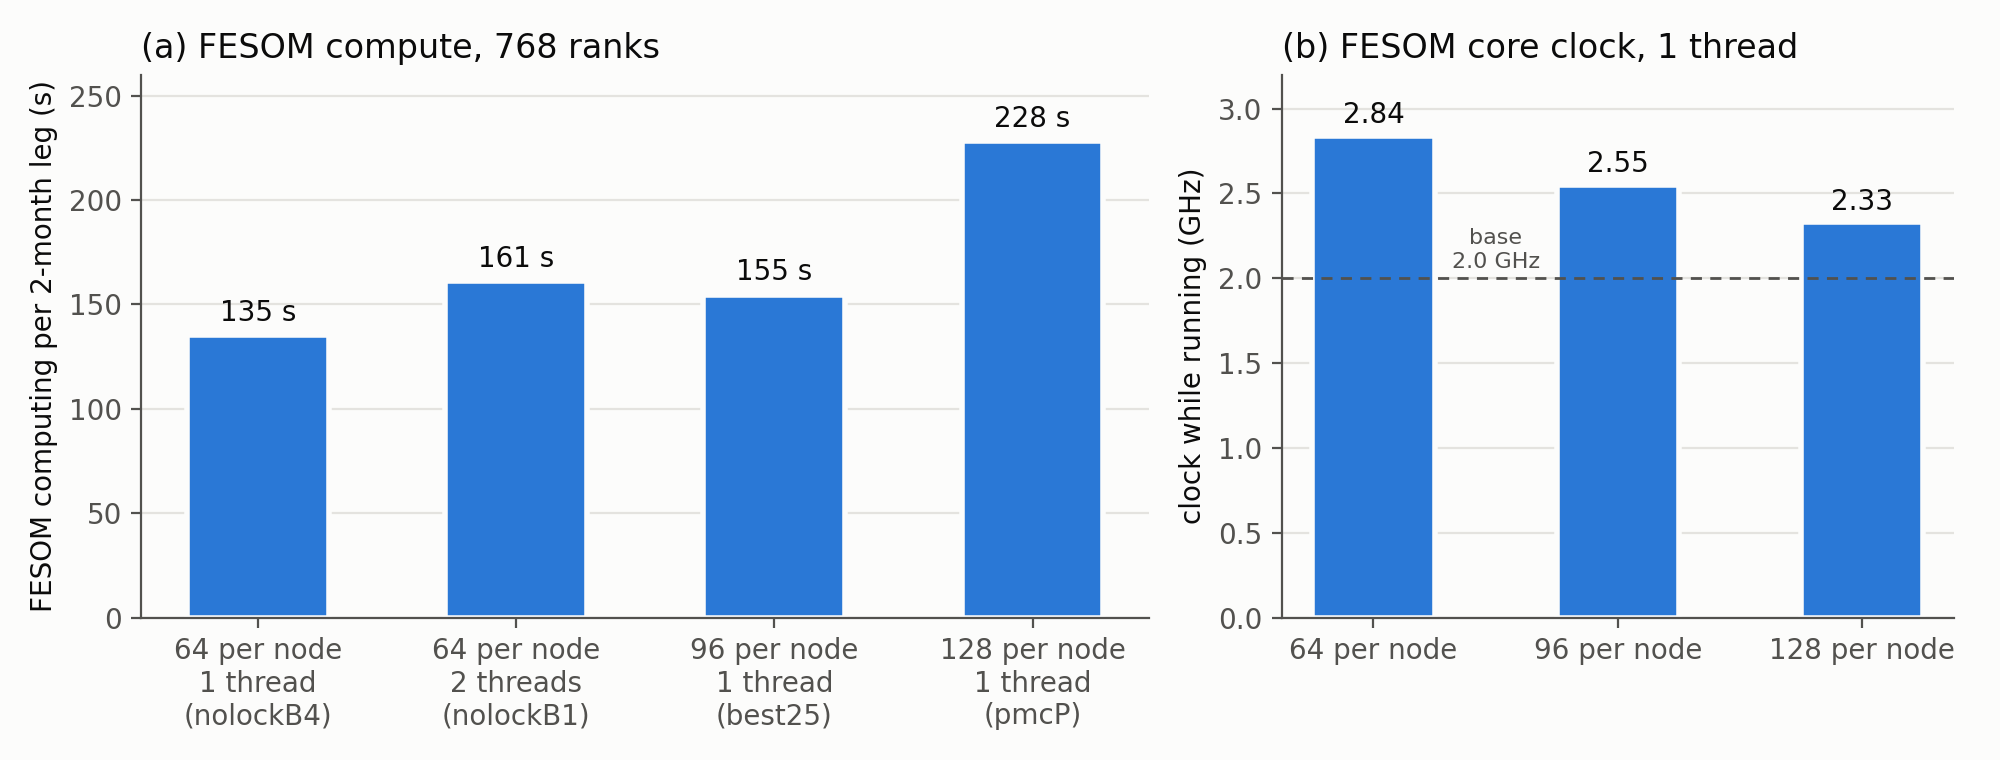
\includegraphics[width=\textwidth]{fig_fesom_spread.png}
\caption{(a) FESOM computing time per 2-month leg (LUCIA timelines) for the same 768 ranks and binary in four layouts. The second OpenMP thread costs 19\,\% against leaving its core idle; packing 128 ranks per node costs 69\,\%. (b) Clock of the busy FESOM cores while they run, from hardware counters: the fewer cores of a node are busy, the higher the rest boost above the 2.0\,GHz base clock. DRAM traffic stays at 40 to 70\,GB/s per node in every layout, far below what a node delivers, so the idle cores buy clock and some cache, not bandwidth.}\label{fig:spread}
\end{figure}

\subsection{Hardware counters: idle neighbours buy clock, not bandwidth (2026-09-29)}
Albedo has neither \texttt{perf} nor likwid, but \texttt{perf\_event\_paranoid}=2 allows user-mode counters on one's own processes. \texttt{bench/pmcwin.c} attaches to every thread of every FESOM and OpenIFS process on a node for 30\,s once OpenIFS has passed model day 10 (started once per node by \texttt{bin/pmcwrap.sh} through \texttt{bin/pmcmon.sh}). It counts task clock, cycles, instructions and three Zen2 events for lines read from DRAM: demand L1D fills (0x43, umask 0x48), L1D hardware-prefetch fills (0x5A, umask 0x48) and L2 prefetches that miss L2 and L3 (0x72). \texttt{bench/pmc\_summary.py} turns them into clock while running, instructions per cycle and DRAM traffic.
\begin{table}[H]\centering\footnotesize\setlength{\tabcolsep}{4pt}
\begin{tabular}{llrrr}\toprule
component & layout (run) & GHz & IPC & DRAM, GB/s per node\\\midrule
FESOM & 64 per node, 1 thread (pmcS, pmcO2) & 2.84 & 1.90 & 39\\
FESOM & 96 per node, 1 thread (fes96) & 2.55 & 1.73 & 66\\
FESOM & 128 per node, 1 thread (pmcP) & 2.33 & 1.71 & $\approx 70$\\
OpenIFS & $384\times4$, 4 threads (pmcS, pmcP, fes96) & 2.44--2.49 & 1.32--1.40 & 19--25\\
OpenIFS & 2 threads on 4 reserved cores (pmcO2) & 2.81 & 1.84 & 21\\
OpenIFS & $768\times2$, 2 threads on 2 cores (oifs768) & 2.41 & 1.54 & 26\\\bottomrule
\end{tabular}
\caption{Counter windows of 30\,s around model day 10. The pmcP value is doubled from 64 sampled of the 128 ranks per node (a limit in the first \texttt{pmcwin}, since fixed). A single busy core on an otherwise idle node ran at 3.28\,GHz.}\label{tab:pmc}
\end{table}
Clock and instructions per cycle together give a spread FESOM rank 1.36 times the instruction rate of a packed one; FESOM's computing time differs by 1.65. The remainder is presumably waiting in MPI, which grows when every rank is slower; the counters cannot show it, since polling also retires instructions. OpenIFS with two threads on its four reserved cores computed as fast as with four (177 against 175\,s): its third and fourth threads contribute nothing at TCO95.

\subsection{Critical path per coupling step (2026-09-29)}
\texttt{bench/lucia\_steps.py} splits the LUCIA timelines into the 1414 coupling intervals of a 2-month leg (one per 3600\,s OpenIFS step, two FESOM steps each) and gives each component's computing and waiting per interval. In pmcS (FESOM 64 per node, 29 nodes, 2.53\,s per model day, about 94\,SYPD in steady state) OpenIFS is the longer component even in its cheapest intervals (88 to 100\,ms against FESOM's 77 to 88), longer still in every third interval, which carries the radiation (115 to 140\,ms), and in one output interval per day (about 210\,ms). FESOM is longer only in its own daily output interval (158\,ms). Summing the longer of the two per interval gives a critical path of 163.0\,s: OpenIFS 10 or 20\,\% faster would shorten it by 7 or 13\,\%, an infinitely fast FESOM by 3\,\%.

\subsection{More OpenIFS ranks, fewer FESOM cores (2026-09-29)}
From the pmcS intervals, fewer FESOM ranks do not pay: at 640, 512 or 384 ranks FESOM would move onto the critical path and cost 6, 21 or 54\,\% in speed for $-1$, $+4$ or $+22$\,\% node-seconds. Fewer cores for the same 768 ranks does: a second option of the placement module, \texttt{ranks\_per\_node} on a component that is not interleaved, starts it on fresh nodes and spreads that many ranks evenly over each node's cores, at 96 per node three of every four, one idle core per L3 group. OpenIFS was tried at $768\times2$ on the same nodes as $384\times4$.
\begin{table}[H]\centering\footnotesize\setlength{\tabcolsep}{4pt}
\begin{tabular}{lllrrrr}\toprule
run & FESOM & OpenIFS & nodes & s per model day & FESOM computing & OpenIFS computing\\\midrule
pmcS & 64 per node & $384\times4$ & 29 & 2.53 & 138.1 & 174.8\\
oifs768 & 64 per node & $768\times2$ & 29 & 3.02 & 141.9 & 197.7\\
fes96 & 96 per node & $384\times4$ & 25 & 2.51 & 158.0 & 173.6\\
fes96o768 & 96 per node & $768\times2$ & 25 & 2.81 & 161.1 & 185.2\\\bottomrule
\end{tabular}
\caption{FESOM $768\times1$ throughout; XIOS four per OpenIFS node. FESOM at 96 per node runs at 2.55\,GHz, computes 14\,\% longer and still stays shorter than OpenIFS, so the model is as fast on 4 fewer nodes. OpenIFS at $768\times2$ packed is slower than $384\times4$ (2.41\,GHz, 1.54 IPC). The running experiments cannot change OpenIFS's decomposition anyway: their OpenIFS restarts are tied to it.}\label{tab:fes96}
\end{table}

\subsection{Production layout (2026-09-29)}
The largest XIOS server grows to 44--46\,GB in a 10-year leg. Four next to 28 OpenIFS ranks of about 3\,GB would need about 268\,GB on a 257\,GB node late in a leg; two per node need about 182\,GB and still fit the 29 nodes. TEST\_prodlayout ran FESOM 64 per node on two reserved cores with one thread, XIOS two per OpenIFS node and rnfmap on an OpenIFS node, with esm\_tools installed into the experiment's own virtual environment from GitHub, as production does: 2.39\,s per model day on 29 nodes, OpenIFS computing 166 against 173\,s in nolockB4 (one run each). TEST\_best25, the same with FESOM at 96 ranks per node, stepped 2.40\,s per model day on 25 nodes: about 99\,SYPD in steady state and 6.1 node-hours per model year, against 14.5 for perfH (47 nodes, 1800\,s) and 19.8 in the first albedo legs (47 nodes, 1200\,s, 4.16\,s per model day).

\begin{figure}[H]\centering
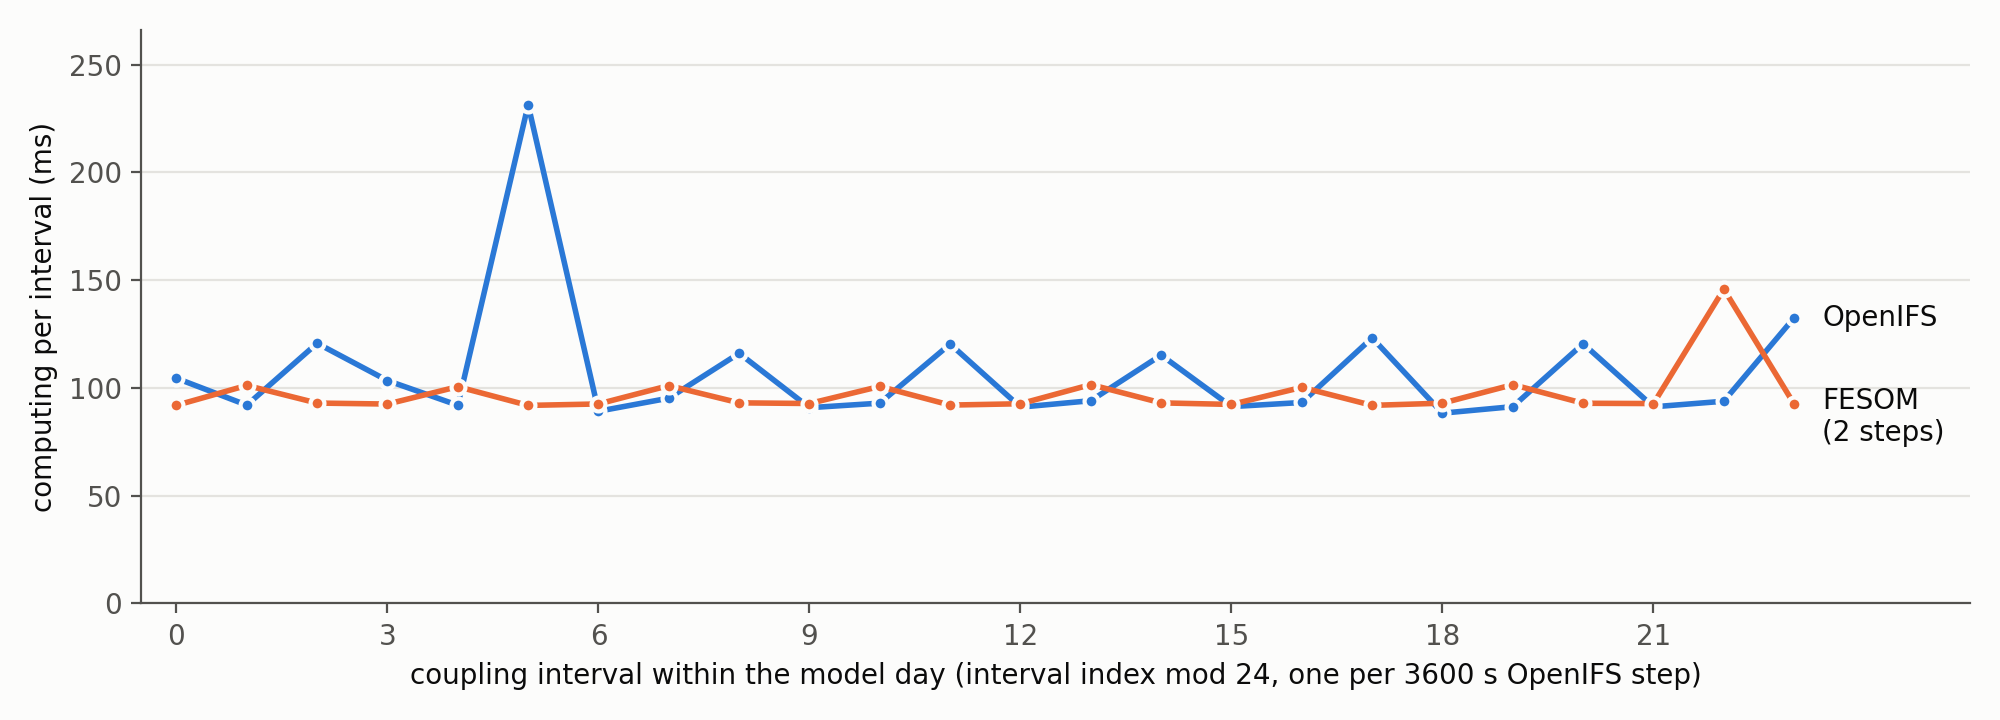
\includegraphics[width=\textwidth]{fig_critical_path.png}
\caption{Computing time per coupling interval in TEST\_best25, averaged over the 59 model days by position in the day. In ordinary intervals FESOM (two steps, 92--102\,ms) is now as long as OpenIFS (88--95\,ms); the long intervals are OpenIFS's radiation steps (every third, 115--133\,ms), one OpenIFS output interval (231\,ms) and one FESOM output interval (146\,ms) per day. FESOM is the longer component in 823 of 1414 intervals. The critical path is 163.7\,s; OpenIFS 20\,\% faster alone would shorten it by 8.5\,\%, an infinitely fast FESOM by 7\,\%.}\label{fig:critpath}
\end{figure}
Both production runscripts (PICAL\_ccnice from leg 2130, PICAL\_crunveg from leg 2120) now use this layout with the 53e095ec build, OpenIFS unchanged at $384\times4$. Their frozen esm\_tools virtual environments (6de9ed453, without the placement module) were moved aside, so the next submission rebuilds them from \texttt{feat/awiesm3-v3.4-co2} at 322f0ed1f. They have not been resubmitted yet.

\section{State of the albedo performance (2026-09-29)}\label{sec:state}
Proven:
\begin{itemize}
\item Albedo runs the same configuration 1.49 times slower than levante (15483 against 10385\,s per 10-year leg).
\item Albedo's cores are 16\,\% slower on cache-resident work; memory bandwidth per core is within 4\,\%.
\item Compute-bound parts are 17 to 29\,\% slower, consistent with the slower cores.
\item Communication-bound parts are 41\,\% (ssh solver) and 83\,\% (ice EVP) slower, the OASIS setup six times.
\item At 1200\,s FESOM limits the coupled model on albedo (LUCIA timelines: FESOM 294\,s, OpenIFS 204\,s computing per 2 months).
\item FESOM's cost per model day doubled since August: 1200\,s instead of 1800\,s time step, TKE+IDEMIX instead of KPP, $K_{GM}$ 2500 instead of 1000.
\item At 1792 ranks FESOM gains only 8\,\% from a second OpenMP thread; at 768 ranks a second thread costs 19\,\% against leaving its core idle.
\item The FESOM time step of 1800\,s gives 72\,SYPD on 47 nodes against 56 at 1200\,s; both production runscripts now use 1800\,s.
\item No MPI setting available on albedo speeds up the model: \texttt{coll/han} and the DC random send policy help the benchmark but not FESOM, RC fails at this size, and HCOLL is not built into any albedo OpenMPI.
\item Inside one node the halo exchange is twice as slow as on levante with every transport available.
\item The initialisation time varies between runs (FESOM setup 14 to 335\,s for identical configurations).
\item CMIP7 output costs 24.5\,\% of OpenIFS CPU and is required.
\item FESOM ranks spend 60 to 75\,\% of the stepping time polling in MPI and 23 to 35\,\% computing, on albedo and on levante alike; ice-free ranks wait longest. Output-mean accumulation costs 7\,\% of FESOM's wall time on both (TEST\_prof).
\item The same 2-month profiling run steps 1.23 times slower on albedo than on levante at 1800\,s; the polling is 1.2 times slower, FESOM's own code 1.1 to 1.7 times.
\item In steady state the machine factor is 1.46 at 1200\,s (10-year legs) and 1.09 at 1800\,s (perfH 3.03 against TEST\_1800 2.77\,s per model day). Over a 2-month leg it is 1.15, because the first model day (OpenIFS cold start) and the last (restart and output writing) take about twice as long on albedo.
\item Levante gains only 2.5\,\% from the 1800\,s FESOM step, albedo 25 to 30\,\%. At 1200\,s FESOM limits on albedo (294 against 204\,s computing per 2 months, LUCIA timelines). At 1800\,s FESOM and OpenIFS compute equally long on both machines (albedo 209 and 209\,s, levante 167 and 171\,s), so a faster FESOM alone gains at most the 37 to 48\,s OpenIFS waits.
\item OpenIFS is 1.22 times and FESOM 1.25 times slower on albedo than on levante in computing time.
\item FESOM \texttt{main} with the OpenMP performance stack (\#1060 merge 1ef85546) computes 13\,\% less at $1792\times1$ and 23\,\% less at $1024\times2$; albedo then steps at 2.72\,s per model day (87\,SYPD steady state), as fast as levante with the old binary, and OpenIFS becomes the limiter.
\item With XIOS packed four servers per node and FESOM at $768\times2$, the model runs on 33 instead of 47 nodes at 2.86\,s per model day (83\,SYPD), 26\,\% fewer node-hours per simulated year; OpenIFS at $192\times8$ is slower than $384\times4$.
\item XIOS servers are busy at most 41\,\%. By memory, four fit on a node of their own, but only two next to OpenIFS ranks over a 10-year leg (44--46\,GB per server).
\item Components can share nodes (esm-tools/esm\_tools\#1603): XIOS and the runoff mapper on the OpenIFS nodes free four nodes at unchanged speed.
\item FESOM runs fastest single-threaded with idle cores next to its ranks: the same 768 ranks compute 135\,s per 2 months at 64 per node, 155 to 158\,s at 96 and 228 to 238\,s at 128. The busy cores run at 2.84, 2.55 and 2.33\,GHz; DRAM traffic of 40 to 70\,GB/s per node is far below what a node delivers.
\item OpenIFS at TCO95 gains nothing from its third and fourth thread (two threads on four reserved cores compute as fast), and $768\times2$ packed is 13\,\% slower than $384\times4$.
\item Production layout: 25 nodes step 2.40\,s per model day, about 99\,SYPD in steady state and 6.1 node-hours per model year (19.8 in the first albedo legs). OpenIFS and FESOM now share the critical path: OpenIFS 20\,\% faster alone would gain 8.5\,\%, an infinitely fast FESOM 7\,\%.
\item After \#1097--\#1099 a rerun at a fixed FESOM thread count is bit-identical; a different thread count still changes the results from the first day.
\end{itemize}
Open:
\begin{itemize}
\item A standalone CORE3 FESOM run on both machines with identical setup would isolate the machine difference from the coupling; levante has CORE3 FESOM 2.6 runs to copy the setup from.
\item Whether the production layout loses speed from spanning several leaf switches (\texttt{no-switch-enforce}); the benchmarks ran within one switch.
\item Whether the intra-node halo penalty is the Zen2 core-complex layout (4 cores per L3 slice against 8 on Zen3); not tested directly.
\item FESOM's timing in Miguel's 100-SYPD runs.
\item Whether FESOM's polling is halo latency, ice load imbalance or the ssh solver's reductions; the sampler records no call stacks. A FESOM rank-count scan (fewer ranks, same layout otherwise) would show how far 1792 ranks are past FESOM's scaling limit.
\item Why EVP on rank 1791 is 2.8 times slower on albedo; first rerun with the same FESOM binary on both machines.
\item Cheaper output-mean accumulation in \texttt{io\_meandata}, and a partition weighted for sea ice.
\item Which code makes the coupled FESOM depend on its thread count; the standalone CI configuration does not.
\item A FESOM partition cut for 96 ranks per node ($n\_part = 8, 96$) instead of \texttt{dist\_768}'s ($12, 64$); it needs its own reordered OASIS set.
\item Speed and XIOS memory of the 25-node layout over a full 10-year leg.
\item OpenIFS's radiation steps and its daily output step now set the pace; the radiation frequency and the FullPos output are the levers on the OpenIFS side.
\end{itemize}

\section{Falsified claims (kept, struck through)}\label{sec:falsified}
\begin{itemize}
\item \dead{OpenIFS computes 0.066\,s and waits 0.089\,s per step (LUCIA summary, TEST\_perfA).} The summary's OpenIFS column is wrong (negative in most runs); the timelines give 186\,s computing and 54\,s waiting for perfA.
\item \dead{FESOM still limits on albedo at 1800\,s.} Also from the LUCIA summary; the timelines show FESOM and OpenIFS computing 209\,s each in perfH.
\item \dead{On levante FESOM does not limit at 1200\,s, so the 1800\,s step gains nothing there.} The evidence was a profiled levante run compared with unprofiled production legs. The unprofiled TEST\_1800 later showed a small gain (2.5\,\%), with FESOM and OpenIFS balanced at 1800\,s, so the conclusion was close but the argument did not hold.
\item \dead{FESOM computes only 84\,\% of the time and has slack, so its cores can be reduced.} The 84\,\% omitted FESOM's output and diagnostics categories; LUCIA shows FESOM computing 91\,\% and waiting 9\,\%.
\item \dead{OpenIFS computes 83\,\% of the time and both models are saturated.} The \texttt{ifs.stat} CPU column includes MPI busy-waiting; LUCIA shows OpenIFS waiting 57\,\% of the time for FESOM.
\item \dead{The initialisation is five times slower than on levante as a property of albedo.} The same files read in 22\,s in TEST\_perfA and FESOM setup ranged from 14 to 335\,s in identical configurations; it varies from job to job.
\item \dead{Give the freed XIOS nodes to OpenIFS, 384 to 768 tasks.} OpenIFS scaling and stability end at about four times the truncation, 380 tasks for TCO95; measured, $768\times2$ on the same nodes computes 13\,\% longer than $384\times4$ (oifs768).
\item \dead{Tidy and file movement make the short legs slow.} Tidy is threaded and takes 20\,s; initialisation takes 5.5\,min.
\item \dead{A precision difference between the machines.} OpenIFS is single precision on both (``The model is using single precision'').
\item \dead{Different FESOM build or namelists.} Namelists are identical and albedo's build targets AVX2 while levante's is generic.
\item \dead{The DC transport's default policy slows FESOM; \texttt{UCX\_TLS=rc\_x,sm,self} or \texttt{UCX\_DC\_MLX5\_TX\_POLICY=rand} fixes it.} Both speed up the benchmark by 2 to 7 times, but RC fails at 2256 ranks and the DC random policy leaves FESOM's EVP and ssh solver unchanged (TEST\_perfG/H).
\item \dead{Hierarchical collectives (\texttt{coll/han}) close the allreduce gap for the ssh solver.} Benchmark allreduce 53 to 24\,$\mu$s, model unchanged (TEST\_perfE/F).
\item \dead{Kernel mitigations make intra-node exchange slow through system calls in CMA/knem.} Transports without system calls (posix, sysv, vader) are as slow or slower than the default.
\item \dead{Albedo's cores are 1.5 to 1.8 times slower on cache-resident code.} Measured 16\,\%.
\item \dead{A GCC build or missing optimisation flags (FESOM PR \#685).} Both machines build with Intel ifort; albedo has more aggressive flags than levante.
\item \dead{FESOM on albedo is limited by memory bandwidth, so spreading its ranks helps by giving each rank more bandwidth.} Hardware counters show 40 to 70\,GB/s of DRAM traffic per node in every layout, far below the node's bandwidth; spread ranks win through clock (2.84 against 2.33\,GHz) and instructions per cycle (1.90 against 1.71).
\item \dead{Removing the OpenMP locks (\#1097--\#1099) makes the coupled model independent of the FESOM thread count.} Reruns become bit-identical, but $768\times2$ and $768\times1$ on the same cores still differ from day 1 (nolockB1, nolockB4).
\item \dead{The lock-free gathers reproduce the old scatter bit for bit at one thread.} The summation order per node is the same by construction, but perfI and nolockI ($1792\times1$, old and new build) differ from day 1 in the coupled model; compiler contraction of multiply-adds is one possible cause, not yet checked.
\end{itemize}

\section{Method notes}
\begin{itemize}
\item OpenIFS wall per step from time stamp differences in \texttt{ifs.stat}; CPU per step is column 5.
\item OpenIFS routine shares from the timing statistics at the end of \texttt{NODE.001\_01}.
\item FESOM: the \texttt{MODEL RUNTIME per task} and \texttt{runtime setup} blocks of rank 0 in the compute log.
\item XIOS: \texttt{Performance report : Ratio} at the end of \texttt{xios\_server*.out} and \texttt{xios\_client*.out}.
\item LUCIA is switched on by \texttt{oasis3mct.use\_lucia: true}, which writes \texttt{\$NLOGPRT 1 0 1} for OASIS3-MCT 5. The result is \texttt{load\_balancing\_info.txt} and \texttt{timeline\_*.nc} in the work directory; \texttt{oasis/util/load\_balancing/pyLucia.py} plots the timelines.
\item The CPU column of \texttt{ifs.stat} includes MPI busy-waiting and must not be read as OpenIFS's compute share.
\item Short tests on albedo: \texttt{compute\_time} of 30\,min or less puts the job into the \texttt{30min} QOS (priority 1 instead of 0).
\item Standalone runs that set \texttt{--cpu\_bind=none} with several OpenMP threads per rank and no \texttt{taskset} leave ranks and threads unpinned; the FESOM 2.8 release tests on 18 nodes collapsed that way (ssh solver 40 to 77 times slower than on one pinned node).
\item Profiling: on levante the sampler's timer signals during start-up broke XIOS's collective \texttt{nc\_create\_par} for the interpolation weights (``Permission denied'' on all FESOM ranks, job 27761837); \texttt{PCS\_DELAY=60} starts the timer after the files are written. \texttt{PCS\_ENABLE=1} and \texttt{LD\_PRELOAD=libpcsampler.so} on selected ranks; \texttt{pcs\_report.py <base> [top] [t0 t1]} restricts to an epoch window. Symbols of stripped libraries (UCX) are only the nearest exported name.
\item Benchmark: \texttt{bench/mpibench.c}; job scripts \texttt{bench/bench\_*.slurm}; the \texttt{HALO\_BYTES} variable sets the halo message size.
\item Seconds per model day: \texttt{bench/ifsstat\_days.awk} on \texttt{ifs.stat}; steady state is the mean of days 2 to 58, since day 1 carries the OpenIFS cold start and the last day the restart writing.
\item Per coupling interval: \texttt{bench/lucia\_steps.py timeline\_OpenIFS.nc timeline\_fesom.nc}; the critical path is the sum over intervals of the longer component.
\item Hardware counters: \texttt{bench/pmcwin.c}, built with \texttt{gcc -O2}, attached by \texttt{bin/pmcmon.sh}, which the wrapper \texttt{bin/pmcwrap.sh} (arguments: thread count, program) starts once per node; summarised by \texttt{bench/pmc\_summary.py} with the work directory as argument. User mode only, so MPI polling in the kernel is not counted but polling in user space is.
\item Fewer threads than reserved cores: set \texttt{omp\_num\_threads} to the cores to reserve and start the program through a wrapper that exports a lower \texttt{OMP\_NUM\_THREADS} (through FESOM's \texttt{execution\_command}, because \texttt{bin\_in\_work} names the staged binary after \texttt{executable}). With \texttt{ranks\_per\_node} the wrapper is no longer needed for FESOM.
\item Bit-comparison of runs: daily FESOM SST, sea-ice concentration and velocity and SSH, compared day by day with \texttt{numpy.array\_equal}.
\end{itemize}

\section{Assets}
\begin{itemize}
\item Runtime: \url{/albedo/work/projects/p_awiesm3_cmip7/jstreffi/runtime/awiesm3-v3.4/}, experiments PICAL\_ccnice, PICAL\_crunveg, TEST\_xiosbus, TEST\_perfA--N, TEST\_placeA/B, TEST\_mevp*, TEST\_nolock*, TEST\_pmc*, TEST\_oifs768, TEST\_fes96*, TEST\_prodlayout, TEST\_best25, TEST\_prof, TEST\_xios1d; failed attempts kept as \texttt{*\_rc\_failed}, \texttt{*\_knobfail}, \texttt{*\_vtune\_ptrace}.
\item Benchmarks, profiler, counter and LUCIA tools, figure script: \texttt{bench/} in this repository, \url{https://github.com/JanStreffing/investigation_awiesm3_albedo_performance}; levante copies in \url{/scratch/a/a270092/lr_probe/}.
\item Wrappers in \url{/albedo/work/user/jstreffi/model_codes/awiesm3-develop/bin/}: \texttt{fesom\_prof.sh}, \texttt{libpcsampler.so}, \texttt{fesom\_omp1.sh}, \texttt{pmcwrap.sh}, \texttt{pmcmon.sh}, \texttt{pmcwin}.
\item FESOM builds in \url{/albedo/work/user/jstreffi/model_codes/awiesm3-develop/fesom-bin/}: \texttt{main1060\_1ef85546} and \texttt{main1060\_53e095ec} (production, libfesom.so md5 18087062).
\item Partitions \texttt{dist\_384}, \texttt{dist\_768}, \texttt{dist\_1024} in \url{/albedo/work/projects/p_awiesm3_cmip7/jstreffi/input/fesom2/core3/}; reordered OASIS sets in \url{/albedo/work/projects/p_awiesm3_cmip7/jstreffi/input/oasis3mct_reorder/}.
\item esm\_tools placement: \url{src/esm_runscripts/placement.py} on branch \url{feat/awiesm3-v3.4-co2} (322f0ed1f) and esm-tools/esm\_tools\#1603.
\item Runscripts: \url{esm_tools/runscripts/awiesm3/develop/awiesm3-develop-albedo-TCO95L91-CORE3_*.yaml} (not committed).
\item Levante reference: \url{/work/bb1469/a270092/runtime/awiesm3-v3.4/PICAL_ccnice/}.
\end{itemize}

\end{document}
